\section {Specification Language} 
\label{sec:ctrt_language}
\begin{figure}[t]
\begin{subfigure}{0.41\textwidth}
\centering
  \begin{fmathpar}
  \begin{array}{lclcl}
		\rel & \in & \texttt{rel.seed} & \coloneqq & \visZ \ALT
		\soZ \ALT \rel \cup \rel \\
               \Rel & \in & \texttt{relation} & \coloneqq &  \rel
	       \ALT \Rel;\rel  \ALT \nullR  \\
	     \pi & \in & \texttt{prop} & \coloneqq & \forall a.
      ~a \xrightarrow{R} \hat{\eff} ~\Rightarrow~ a \xrightarrow{\visZ}
      \hat{\eff}\\
		\psi & \in & \texttt{spec} & \coloneqq & \pi \ALT \pi \conj \pi
  \end{array}
  \end{fmathpar}
\subcaption{ syntax of contracts}
\label{fig:ctrt_syntax}
\end{subfigure}
\hfill \vline \hfill
\begin{subfigure}{0.49\textwidth}
\centering
\begin{scriptsize}
\begin{tabular}{|l | c |} 
\hline
 { \texttt Guarantee} & {\texttt Contract} \\ [0.5ex] 
\hline 
\textsc{Read My Writes} & $\forall a. a ~  ~\xrightarrow{\soZ}  ~ ~
\hat{\eta} \Rightarrow a \xrightarrow{\visZ} \hat{\eta} $ \\ 
\textsc{Monotonic Writes} & $\forall a. a \xrightarrow{\soZ;\visZ}
\hat{\eta} \Rightarrow a \xrightarrow{\visZ} \hat{\eta} $ \\ 
\textsc{Monotonic Reads} & $\forall a. a \xrightarrow{\visZ;\soZ}
\hat{\eta} \Rightarrow a \xrightarrow{\visZ} \hat{\eta} $ \\ 
\textsc{Transitive Visibility} & $\forall a. a \xrightarrow{\visZ;\visZ}
\hat{\eta} \Rightarrow a \xrightarrow{\visZ} \hat{\eta} $ \\ 

\hline
\end{tabular}
\end{scriptsize}
\subcaption{examples 
%({\bf R}ead {\bf M}y {\bf W}rites, {\bf M}onotonic
%{\bf W}rites and
%{\bf M}onotonic {\bf R}eads)
}
\label{fig:ctrt_example}
\end{subfigure}
\caption{\tool Specification Language}
\end{figure}


The formal syntax of our specification language is presented in
Fig.~\ref{fig:ctrt_syntax}.  The language allows the definition of
propositions, FOL formulae that establish the conditions under which
one effect may become visible to another.  The dependencies that must
hold for a particular visibility effect to be valid is given in
terms of a composition of 

The type \relationS{} which is used to define dependencies between
effects in \propS{}s, is a sequence of \seedS{}s where each of them is
a $\visZ$ or $\soZ$ relation or the union of them both over the set of
effects. In order to configure each environment, the developers are
required to write a \specS{} for each of them, that is consisted of
conjunctions of \propS{}s, which simply allows developers to
eliminiate multiple types of anomalous behavior from each
environment. For example, the developers of the comment management
application, can simply write $\psi_1\wedge \psi_2$ for their \readC{}
operation and prevent \emph{both} anomalies explained in the previous
section.

Now we syntactically  classify propositions into \emph{lower bound} (LB) and
\emph{upper bound} (UB) and hybrid types, and show that they completely
align with types of
anomalies previously mentioned. 
\begin{itemize}
\item {\bf LB}: We define a \propS{} to be of type LB, 
if its dependency relation $R$, ends with an $\soZ$ relation, i.e. is of
the following from: $\forall(\eff,\eff'). \eff \xrightarrow{r_1;r_2;...;\soZ} \eff'
\Rightarrow \eff \xrightarrow{\visZ} \eff'$.
Observe that these contracts simply put a lower bound on the set of
effects each operation must witness, by defining a certain set of
dependency for each effect, that must be visible to it, which makes the
blocking technique very suitable for easily maintaining them.
\item {\bf UB}:  These propositions are similarly defined as \propS{}s
with dependency relations ending with $\visZ$, or of the following form: 
$\forall(\eff,\eff'). \eff \xrightarrow{r_1;r_2;...;\visZ} \eff'
\Rightarrow \eff \xrightarrow{\visZ} \eff'$.
This type of \propS{}s, put an upper bound on the set of effects 
a replica should make visible to each operation when executing it, by
enforcing that if an effect is made visible, certain set of dependent
effects must also be made visible. This clearly resembles the
filteration technique, where only a subset of available effects can enter
the consistent environments.
\item {\bf Hybrid}: The \propS{}s whose dependency relation ends with
$\visZ\cup \soZ$, which require both blocking and filteration to be
maintained. 
\end{itemize}
We can extend the above definitions to \specS{}s also, by defining an LB
(UB) \specS{} to contain only LB (UB) \propS{}s. Hybrid \specS{}s are also
defined as the ones that are neither LB or UB.

We finish this section by presenting weak consistency guarantees from
Terry et. al. in figure \ref{fig:ctrt_rep}, which shows the generality
of our simple specification language. We also present a simple way of
representing contracts as graphs where the left-hand-side of the
contracts are depicted as the sequence of edges relating two effects,
and the right-hand-sinde (or what must be enforced by replicas at the
execution time) is represented as the single dashed $\visZ$ edge.
\begin{figure}[t]
        \centering
	\begin{subfigure}[b]{0.3\textwidth}
	\caption{Read My Writes: \\
	$\forall(\eff,\eff'). \eff \xrightarrow{\soZ} \eff \Rightarrow
	\eff \xrightarrow{\visZ} \eff'$}
	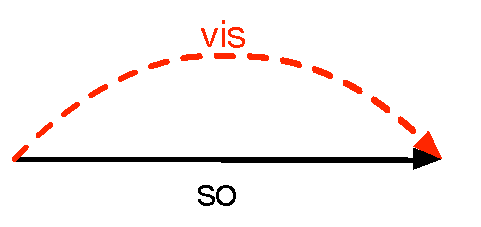
\includegraphics[scale=0.5]{Figures/rmw.pdf}
	\end{subfigure}
	%
	\vrule
	\hfill
	\begin{subfigure}[b]{0.3\textwidth}
	\caption{Monotonic Reads: 
	\\	$\forall(\eff,\eff'). \eff \xrightarrow{\visZ;\soZ} \eff \Rightarrow
	\eff \xrightarrow{\visZ} \eff' $}
	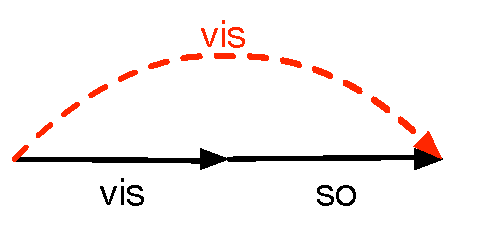
\includegraphics[scale=0.5]{Figures/mr.pdf}
	\end{subfigure}
	%
	\vrule
	\hfill
	\begin{subfigure}[b]{0.25\textwidth}
	\caption{Monotonic Writes:
	\\	$\forall(\eff,\eff'). \eff \xrightarrow{\soZ;\visZ} \eff \Rightarrow
	\eff \xrightarrow{\visZ} \eff' $}
	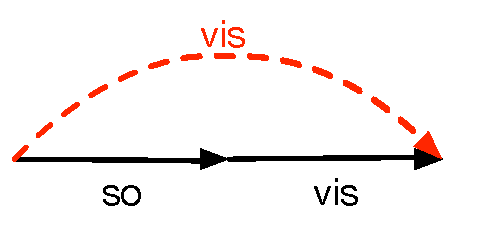
\includegraphics[scale=0.5]{Figures/mw.pdf}
	\end{subfigure}
	%
%	\begin{subfigure}[b]{0.24\textwidth}
%	\centering
%	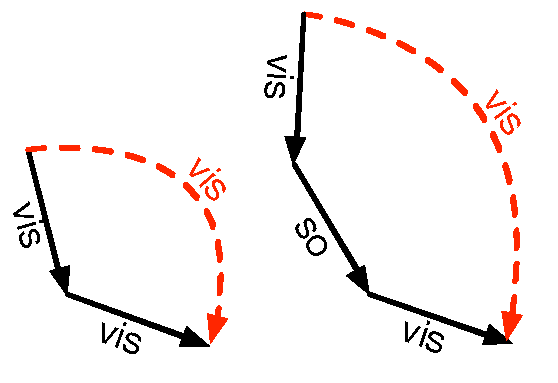
\includegraphics[scale=0.38]{Figures/wfr.pdf}
%	\caption{Writes Follow Reads}
%	\end{subfigure}
\\ \hrulefill

\caption{Known weak consistency guarantees written in our specification
language}
\label{fig:ctrt_rep}
\end{figure}



